% TFF-Title: Maze with highlighted solution path
% TFF-Family: decorative
% TFF-Tags: maze, path, grid, routing, decorative
% TFF-Description: Maze-style wall drawing with a clearly separated start-to-target solution route.
% TFF-Origin: https://texample.net/maze/
% TFF-License: CC BY-SA 4.0
% TFF-Attribution: Adapted from the PGF/TikZ manual maze example as published on TeXample.net
\documentclass[tikz,border=7pt]{standalone}
\usetikzlibrary{arrows.meta}
\begin{document}
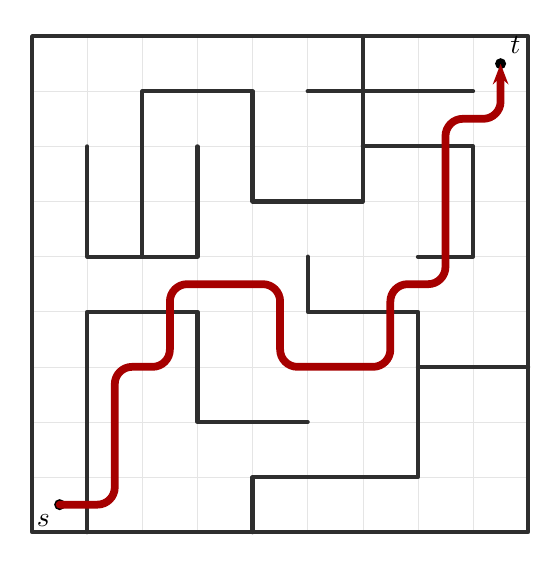
\begin{tikzpicture}[x=7mm,y=7mm]
  \draw[step=1,help lines,draw=black!10] (-2,-2) grid (7,7);
  \tikzset{wall/.style={draw=black!82,line width=1.5pt,line cap=round,line join=round}}
  \draw[wall] (-2,-2) rectangle (7,7);
  \draw[wall] (-1,-2)--(-1,2)--(1,2)--(1,0)--(3,0);
  \draw[wall] (0,3)--(0,6)--(2,6)--(2,4)--(4,4)--(4,7);
  \draw[wall] (2,-2)--(2,-1)--(5,-1)--(5,2)--(3,2)--(3,3);
  \draw[wall] (5,1)--(7,1);
  \draw[wall] (5,3)--(6,3)--(6,5)--(4,5);
  \draw[wall] (1,5)--(1,3)--(-1,3)--(-1,5);
  \draw[wall] (3,6)--(6,6);
  \coordinate (s) at (-1.5,-1.5);
  \coordinate (t) at (6.5,6.5);
  \fill (s) circle (2pt) node[below left] {$s$};
  \fill (t) circle (2pt) node[above right] {$t$};
  \draw[-{Stealth[length=2.6mm]},draw=red!65!black,line width=2.8pt,
        rounded corners=2.2mm,line cap=round,line join=round]
    (s)--(-.5,-1.5)--(-.5,1)--(.5,1)--(.5,2.5)--(2.5,2.5)
       --(2.5,1)--(4.5,1)--(4.5,2.5)--(5.5,2.5)--(5.5,5.5)
       --(6.5,5.5)--(t);
\end{tikzpicture}
\end{document}
